\documentclass[14pt, a4paper]{extarticle}
\usepackage{style}
\usepackage{array}
\usepackage{biblatex}
\usepackage{amsmath}
\usepackage{indentfirst}
\usepackage{listings}
\usepackage{xcolor}
\usepackage{fefutitle}
\usepackage[justification=centering]{caption}
\usepackage{float}

\lstdefinestyle{mystyle}{
	basicstyle={\small\ttfamily},
	keywordstyle=\color{orange},
	stringstyle=\color{green},
	basicstyle=\ttfamily\footnotesize,
	breakatwhitespace=false,         
	breaklines=true,                 
	captionpos=b,                    
	keepspaces=true,                 
	numbers=none,                    
	numbersep=5pt,                  
	showspaces=false,                
	showstringspaces=false,
	showtabs=false,                  
	tabsize=2,
	aboveskip=3mm,
	belowskip=3mm,
	frame=single
}
\lstset{style=mystyle}
\newcolumntype{P}[1]{>{\centering\arraybackslash}p{#1}}

\begin{document}
	
	\fefutitle{2}{Метод вырожденных ядер для решения уравнения Фредгольма 2-го рода}
	\pagebreak
	
	\pagebreak
	
	\section{Введение}
	
	Объектом исследования являются численные методы решения задач математической физики, а также программное обеспечение, реализующее эти методы.
	
	Цель работы – ознакомиться с численными методами решения задач математической физики решить предложенные типовые задачи, сформулировать выводы по полученным решениям, отметить достоинства и недостатки методов, сравнить удобство использования и эффективность работы каждой использованной программы, приобрести практические навыки и компетенции, а также опыт самостоятельной профессиональной деятельности, а именно:
	
	\begin{itemize}
		\item создать алгоритм решения поставленной задачи и реализовать его, протестировать программы;
		
		\item освоить теорию вычислительного эксперимента; современных компьютерных технологий;
		
		\item приобрести навыки представления итогов проделанной работы в виде отчета, оформленного в соответствии с имеющимися требованиями, с привлечением современных средств редактирования и печати.
		
	\end{itemize}

	Работа над курсовым проектом предполагает выполнение следующих задач:
	
	\begin{itemize}
		\item дальнейшее углубление теоретических знаний обучающихся и их систематизацию;
		
		\item получение и развитие прикладных умений и практических навыков по направлению подготовки;
		
		\item овладение методикой решения конкретных задач;
		
		\item развитие навыков самостоятельной работы;
		
		\item развитие навыков обработки полученных результатов, анализа и осмысления их с учетом имеющихся литературных данных;
		
		\item приобретение навыков оформления описаний программного продукта;
		
		\item повышение общей и профессиональной эрудиции.
		
	\end{itemize}

	Изученный студентом в ходе работы материал должен способствовать повышению его качества знаний, закреплению полученных навыков и уверенности в выборе путей будущего развития своих профессиональных способностей. 
	
	\section{Основная часть}
	\subsection{Постановка задачи}
		Интегральные уравнения -- функциональное уравнение, которое содержит интегральное преобразование над искомой функцией.
		
		В достаточно общем случае линейные интегральные уравнения могут быть представлены в виде
		\[ g(x)y(x) - \lambda \int\displaylimits_{\Omega} K(x, s)y(s)ds = f(x), x \in Q \]
		, где $K(x, s)$ - ядро, $f(x)$ - правая часть уравнения с область определения $Q$, $\lambda$ - параметр уравнения, $y(s)$ - искомая функция с область определения $\Omega$.
		
		Если $\Omega$ постоянная и $g(x) \neq 0$, то интегральное уравнение в этом случае есть уравнение Фредгольма 2-го рода
		\begin{equation}
			y(x) - \lambda \int\displaylimits_{a}^{b} K(x,s)y(s)ds = f(x)
			\label{eq:1}
		\end{equation}
		
		В данной курсовой работе решение уравнения Фредгольма 2-го рода будем искать с помощью метода вырожденных ядер.
	\subsection{Описание алгоритма решения задачи}
		Ядро $K(x,s)$ называется вырожденным, если оно представимо в виде
		\[ K(x,s) \approx \sum_{i=1}^{n} \alpha_i(x) \beta_i(s) \]
		, где функции $\alpha_i(x)$ и $\beta_i(s)$ линейно независимы на отрезке $[a, b]$.
		
		Данный метод основан на том, что для интегрального уравнения с вырожденным ядром может быть получено точное решение. Заменим в \ref{eq:1} ядро $K(x, s)$ вырожденным
		\begin{equation}
			y(x) - \lambda \int\displaylimits_{a}^{b} \bigg[\sum_{i=1}^{n} \alpha_i(x) \beta_i(s)\bigg] y(s)ds = f(x)
			\label{eq:2}
		\end{equation}
		
		\[ y(x) - \lambda \sum_{i=1}^{n} \alpha_i(x) \int\displaylimits_{a}^{b} \beta_i(s)y(s)ds = f(x) \]
		Если обозначить 
		\[ \int\displaylimits_{a}^{b} \beta_i(s)y(s) = C_i \]
		, то можно получить следующую форму решения:
		\begin{equation}
			y(x) = f(x) + \lambda \sum_{i=1}^{n} C_i \alpha_i(x)
			\label{eq:3}
		\end{equation}
		Подставляя \ref{eq:3} в \ref{eq:2}, получим:
		\[ C_i - \lambda \sum_{j=1}^{n} C_j\int\displaylimits_{a}^{b} \alpha_j(s)\beta_j(s)ds = \int\displaylimits_{a}^{b} \beta_i(s)f(s)ds \]
		\pagebreak
		Если ввести обозначения,
		\[ A_{ij} = \int\displaylimits_{a}^{b} \alpha_j(s)\beta_j(s)ds \]
		\[ f_{ij} = \int\displaylimits_{a}^{b} \beta_i(s)f(s)ds \]
		, получим
		\[ C_i - \lambda \sum_{j=1}^{n} A_{ij}C_j = f_i \]
		
		Получаем СЛАУ относительно $C_i$. Решив эту систему получим решение уравнения в виде \ref{eq:3}.
		Если ядро не является вырожденным, то его можно аппроксимировать таковым и, применив данный метод, получить приближенное решение. В данной работе для аппроксимации ядра будет использовать первые 3 члена разложения в ряд Тейлора и аппроксимация интерполяционным многочленом Лагранжа с помощью 3 точек.
			
	\subsection{Описание тестов, использованных для отладки}
		Для тестов было выбрано следующее интегральное уравнения с известным точным решением:
		\[ y(x) - \int\displaylimits_{0}^{1} x^2 \cos{(xs)} y(s)ds = x - x\sin{x} - \cos{x} + 1, \; y = x \]
		\begin{figure}[h]
			\centering
			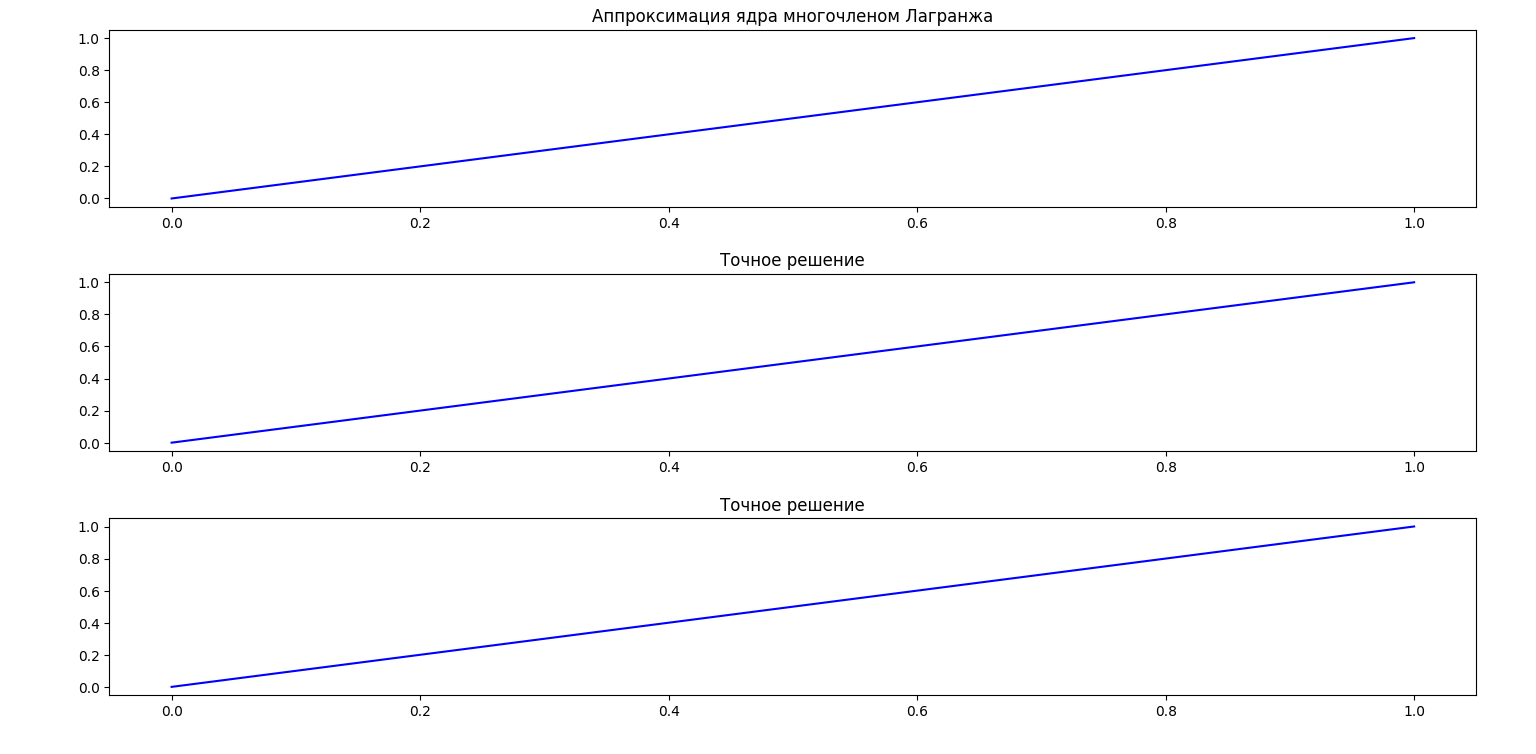
\includegraphics[width = \linewidth]{plot_1.png}
			\caption{Графики решения ИУ}
		\end{figure}
		\begin{center}
			\begin{tabular}{ |c|c|c|c| }
				\hline
				$x$ & Точное решение & Лагранж & Тейлор\\
				\hline
				0 & 0 & 0 & 0\\
				\hline
				0,1 & 0,1 & 0,1 & 0,1\\
				\hline
				0,2 & 0,2 & 0,2 & 0,2\\
				\hline
				0,3 & 0,3 & 0,29999 & 0,3\\
				\hline
				0,4 & 0,4 & 0,4 & 0,4\\
				\hline
				0,5 & 0,5 & 0,5 & 0,5\\
				\hline
				0,6 & 0,6 & 0,6 & 0,60001\\
				\hline
				0,7 & 0,7 & 0,69999 & 0,70002\\
				\hline
				0,8 & 0,8 & 0,8 & 0,80004\\
				\hline
				0,9 & 0,9 & 0,9 & 0,90008\\
				\hline
				1 & 1 & 1 & 1,0001\\
				\hline
			\end{tabular}
		\end{center}
	\pagebreak
	\subsection{Вычислительные эксперименты}
	\[ y(x) - \int\displaylimits_{0}^{1} \dfrac{\sin{(0.6xs)}}{s}y(s)ds = x \]
	\begin{figure}[h]
		\centering
		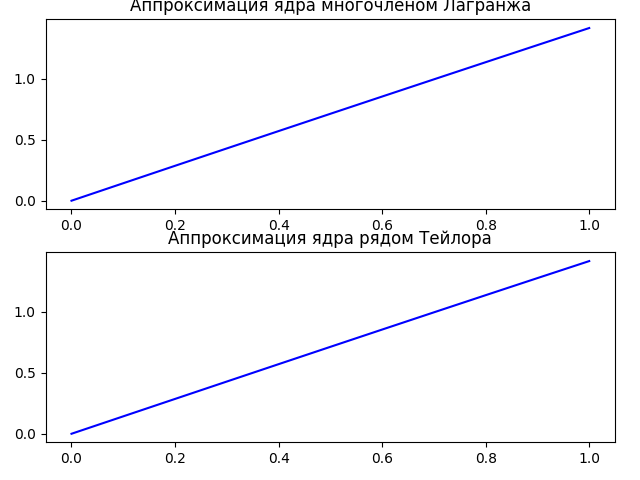
\includegraphics[width = \linewidth]{plot_2.png}
		\caption{Графики решения ИУ}
	\end{figure}
	\begin{center}
		\begin{tabular}{ |c|c|c| }
			\hline
			$x$ & Лагранж & Тейлор\\
			\hline
			0 & 0 & 0\\
			\hline
			0,1 & 0,14302 & 0,14257\\
			\hline
			0,2 & 0,28566 & 0,28506\\
			\hline
			0,3 & 0,42793 & 0,42741\\
			\hline
			0,4 & 0,56981 & 0,56952\\
			\hline
			0,5 & 0,56982 & 0,56952\\
			\hline
			0,6 & 0,85247 & 0,85277\\
			\hline
			0,7 & 0,99324 & 0,93375\\
			\hline
			0,8 & 1,13362 & 1,13420\\
			\hline
			0,9 & 1,27362 & 1,27406\\
			\hline
			1 & 1,41326 & 1,41325\\
			\hline
		\end{tabular}
	\end{center}

	\[ y(x) - \int\displaylimits_{0}^{1} \dfrac{xs}{1+0.1xs} y(s)ds = e^{-x} \]
	\begin{figure}[h]
		\centering
		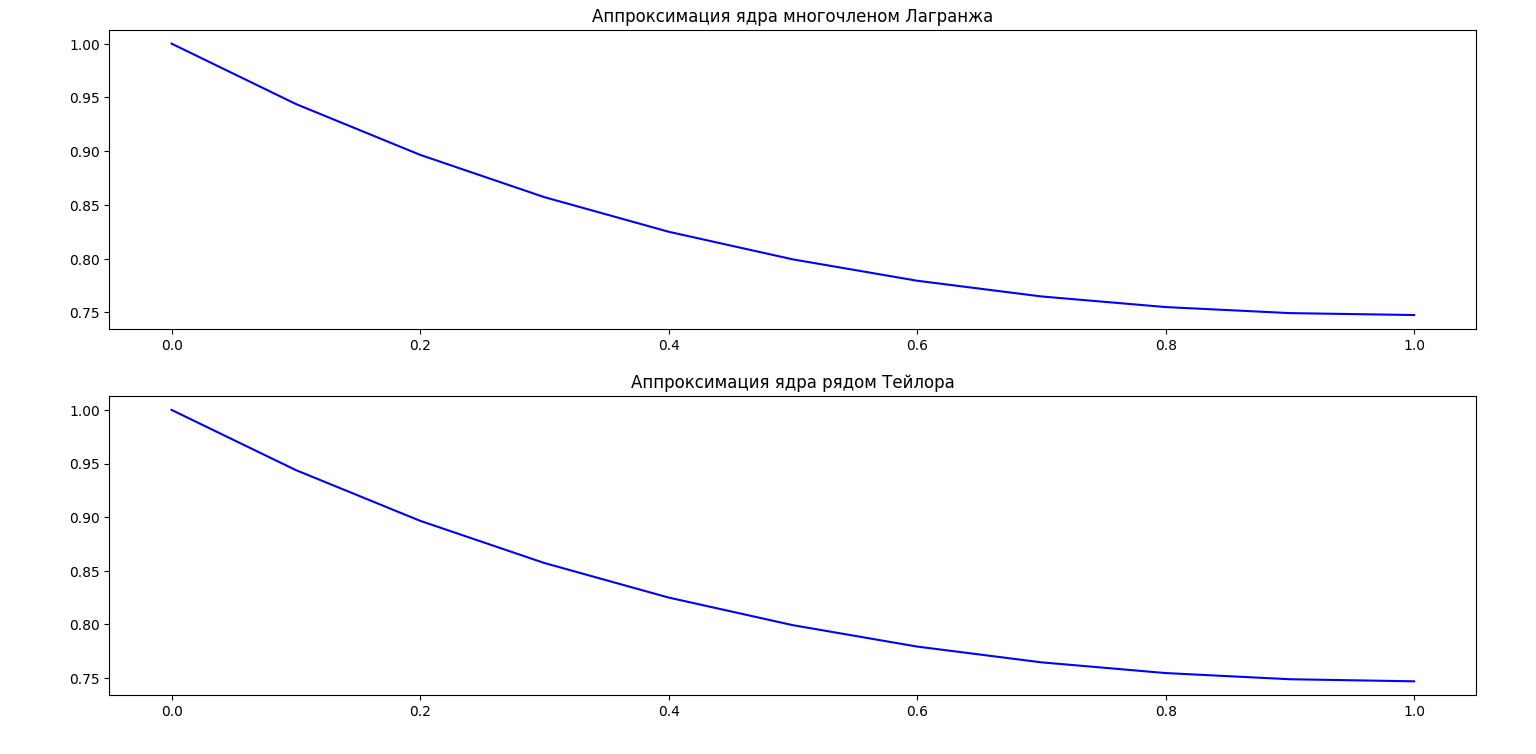
\includegraphics[width = \linewidth]{plot_3.png}
		\caption{Графики решения ИУ}
	\end{figure}
	\begin{center}
		\begin{tabular}{ |c|c|c| }
			\hline
			$x$ & Лагранж & Тейлор\\
			\hline
			0 & 1 & 1\\
			\hline
			0,1 & 0,94386 & 0,94386\\
			\hline
			0,2 & 0,89654 & 0,89653\\
			\hline
			0,3 & 0,85718 & 0,85714\\
			\hline
			0,4 & 0,82500 & 0,82491\\
			\hline
			0,5 & 0,79930 & 0,79913\\
			\hline
			0,6 & 0,77942 & 0,77917\\
			\hline
			0,7 & 0,76480 & 0,76444\\
			\hline
			0,8 & 0,75492 & 0,75444\\
			\hline
			0,9 & 0,74930 & 0,74868\\
			\hline
			1 & 0,74751 & 0,74673\\
			\hline
		\end{tabular}
	\end{center}
	
	\[ y(x) - \int\displaylimits_{0}^{1} (1+s)(e^{0.2xs}-1)y(s)ds = \dfrac{1}{x} \]
	\begin{figure}[h]
		\centering
		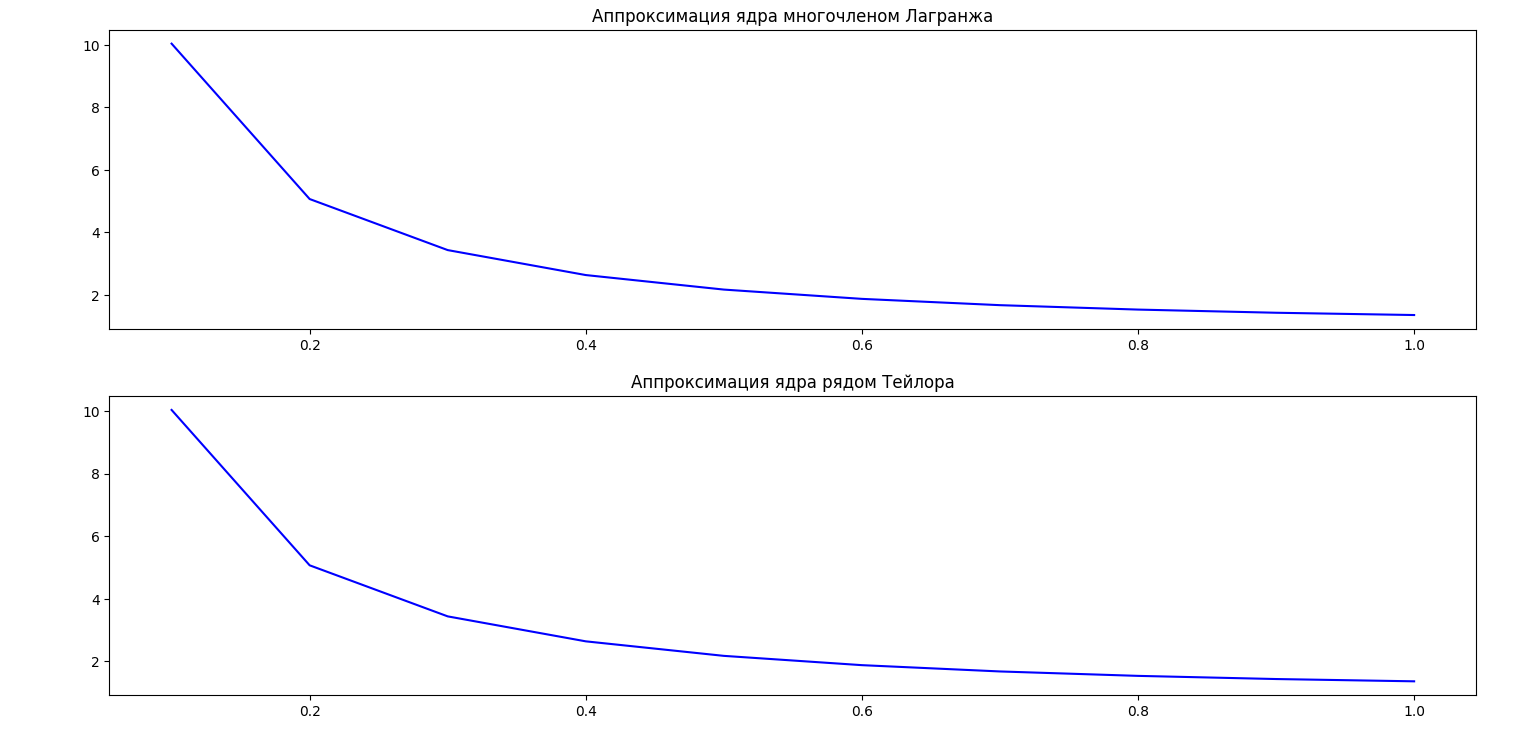
\includegraphics[width = \linewidth]{plot_4.png}
		\caption{Графики решения ИУ}
	\end{figure}
	\begin{center}
		\begin{tabular}{ |c|c|c| }
			\hline
			$x$ & Лагранж & Тейлор\\
			\hline
			0 & $\infty$ & $\infty$\\
			\hline
			0,1 & 10,03433 & 10,03437\\
			\hline
			0,2 & 5,06910 & 5,06914\\
			\hline
			0,3 & 3,42762 & 3,43766\\
			\hline
			0,4 & 2,63991 & 2,63993\\
			\hline
			0,5 & 2,17596 & 2,17595\\
			\hline
			0,6 & 1,87910 & 1,87906\\
			\hline
			0,7 & 1,67791 & 1,67784\\
			\hline
			0,8 & 1,53667 & 1,53658\\
			\hline
			0,9 & 1,43554 & 1,435456\\
			\hline
			1 & 1,362622 & 1,36255\\
			\hline
		\end{tabular}
	\end{center}
		
	\section{Заключение}
	
	В результате работы над курсовым проектом были реализованы метод вырожденных ядер для решения уравнения Фредгольма 2-го рода. Метод были протестирован и отлажены на тестовом примере, а затем применен для вычислительных экспериментов.
	
	Приобрел практические навыки владения:
	
	\begin{itemize}
	\item современными численными методами решения задач линейной алгебры;
	
	\item основами алгоритмизации для численного решения задач линейной алгебры на языке программирования Python 3;
	
	\item инструментальными средствами, поддерживающими разработку программного обеспечения для численного решения задач линейной алгебры;
	
	\end{itemize}
	а также навыками представления итогов проделанной работы в виде отчета, оформленного в соответствии с имеющимися требованиями, с привлечением современных средств редактирования и печати.
	\section{Список использованных источников}
	\begin{enumerate}
		\item Верлань А.Ф. Интегральные уравнения: методы, алгоритмы, программы/ А.Ф. Верлань, В.С. Сизиков -- Киев: Наукова думка, 1986 г. – 544 с.
		
		\item Колобов А.Г. Лабораторные работы по Численным методам / А.Г. Колобов, Л.А. Молчанова -- Владивосток: Изд-во Дальневост. ун-та, 2007 г. - 36 с.
	\end{enumerate}
	
	\section{Приложения (тексты программ)}
		\lstinputlisting[language=Python]{./lab_5.py}		
\end{document}} 
